\documentclass{article}
\usepackage{algorithm}
\usepackage{algpseudocode}
\usepackage{amsmath,amssymb,amsthm}
\usepackage{graphicx}
\usepackage[margin=1in]{geometry}
\usepackage{fancyhdr}
\usepackage{float}
\usepackage{longtable}
\newcommand{\bx}{{\bf x}}
\newcommand{\bw}{{\bf w}}
\newcommand{\bb}{{\bf b}}
\newcommand{\bv}{{\bf v}}
\newcommand{\by}{{\bf y}}
\setlength{\parindent}{0pt}
\setlength{\parskip}{5pt plus 1pt}
\setlength{\headheight}{13.6pt}
\newcommand\question[2]{\vspace{.25in}\hrule\textbf{#1: #2}\hrule\vspace{.10in}}
\renewcommand\part[1]{\vspace{.10in}\textbf{(#1)}}
\newcommand\algo{\vspace{.10in}\textbf{Algorithm: }}
\newcommand\correctness{\vspace{.10in}\textbf{Correctness: }}
\newcommand\runtime{\vspace{.10in}\textbf{Running time: }}
\newcommand\pseudoCode{\vspace{.10in}\textbf{PseudoCode: }}
\newcommand*{\perm}[2]{{}^{#1}\!P_{#2}}
\newcommand*{\comb}[2]{{}^{#1}\!C_{#2}}
%\pagestyle{fancyplain}
%\lhead{\textbf{\NAME\ (\UID)}}
%\chead{\textbf{Hw\HWNUM}}
%\rhead{CS 6350, \today}
\title{CS6210 - Homework/Assignment-6}
\author{Arnab Das(u1014840)}
\usepackage[utf8]{inputenc}
\begin{document}
  \pagenumbering{gobble}
  \maketitle
  \newpage
  \pagenumbering{arabic}
  \newcommand\NAME{ARNAB DAS}
  \newcommand\UID{uxxxxxxx}
  \newcommand\HWNUM{4}


  \question{Question-1}{Chapter-13, question-5}
  \part{a} Given function, $f(t) = e^{-3t}$ on the interval [0,3]. Let $q_2(t)$ be the approximation of degree 2 and $q_3(t)$ be the approximation of degree 3. \newline
  Let $\phi_0(t), \phi_1(t), \phi_2(t), \phi_3(t)$ be the polynomial basis functions.
  We use the affine transformation to map them to the legendre polynomials as:
  \[x = \dfrac{2t -a -b}{b-a} = \dfrac{2t - 3}{3}\]
  Then , the basis functions in form of legendre polynomials become:
  \[ \phi_0(t) = 1\]
  \[ \phi_1(t) = \dfrac{2t-3}{3}\]
  \[ \phi_2(t) = \dfrac{1}{2}[3\bigg (\dfrac{2t-3}{3}\bigg )^2 - 1]\]
  \[ \phi_3(t) = \dfrac{1}{2}[5\bigg (  \dfrac{2t-3}{3}\bigg )^3 - 3\dfrac{2t-3}{3}]\]

   \textbf{Note:} The evaluations are done in matlab. \newline
  Next, we need to evaluate the matrix elements $B(j,k) = \int_{a}^{b}\phi_j(x)\phi_k(x)$. Since, the basis are orthogonal as we have chosen Legendre polynomials, hence we have only the diagonal elements: Thus:
  \[ B_{0,0} = \int_{0}^{3} \phi_0(t)\phi_0(t) dt = 3 \]
  \[ B_{1,1} = \int_{0}^{3} \phi_1(t)\phi_1(t) dt = 1 \]
  \[ B_{2,2} = \int_{0}^{3} \phi_2(t)\phi_2(t) dt = 0.6 \]
  \[ B_{3,3} = \int_{0}^{3} \phi_3(t)\phi_3(t) dt = 0.4280 \]

  Next, evaluate the $b$ vector of the rhs whose elements are defined as: $b_j = \int_{a}^{b} \phi_j(t)f(t) dt$
  \[b_0 = \int_{0}^{3} \phi_0(t)f(t) dt = 0.3333\]
  \[b_1 = \int_{0}^{3} \phi_1(t)f(t) dt = -0.2593\]
  \[b_2 = \int_{0}^{3} \phi_2(t)f(t) dt = 0.1604\]
  \[b_3 = \int_{0}^{3} \phi_3(t)f(t) dt = -0.0811\]

  Then, we can get the coefficients as: $c_j = \dfrac{b_j}{B_{j,j}}$ 
  \[c_0 = \dfrac{b_0}{B_{0,0}} = 0.111\]
  \[c_1 = \dfrac{b_1}{B_{1,1}} = -0.2593\]
  \[c_2 = \dfrac{b_2}{B_{2,2}} = 0.2674\]
  \[c_3 = \dfrac{b_3}{B_{3,3}} = -0.1892\]

  Hence, the quadratic will be:
  \[q_2(t) = c_0\phi_0(t) + c_1\phi_1(t) + c_2\phi_2(t) = 0.111 - 0.2593(\dfrac{2t-3}{3}) + 0.2674\dfrac{1}{2}[3\bigg (\dfrac{2t-3}{3}\bigg )^2 - 1]\]

  And the cubic will be:
  \[q_3(t) = c_0\phi_0(t) + c_1\phi_1(t) + c_2\phi_2(t) + c_3\phi_3(t) \] \[ 0.111 - 0.2593(\dfrac{2t-3}{3}) + 0.2674\dfrac{1}{2}[3\bigg (\dfrac{2t-3}{3}\bigg )^2 - 1] -0.1892\dfrac{1}{2}[5\bigg (  \dfrac{2t-3}{3}\bigg )^3 - 3\dfrac{2t-3}{3}]\]
	The code implementation is in Prob1.m

  \part{b} The below figure shows the plots for the qudratic, cubic and original plot in the first subplot, and the error plots for quadratic and cubic with respect to the orginal, in the second subplot.
  \begin{figure}[H]
   \centering
  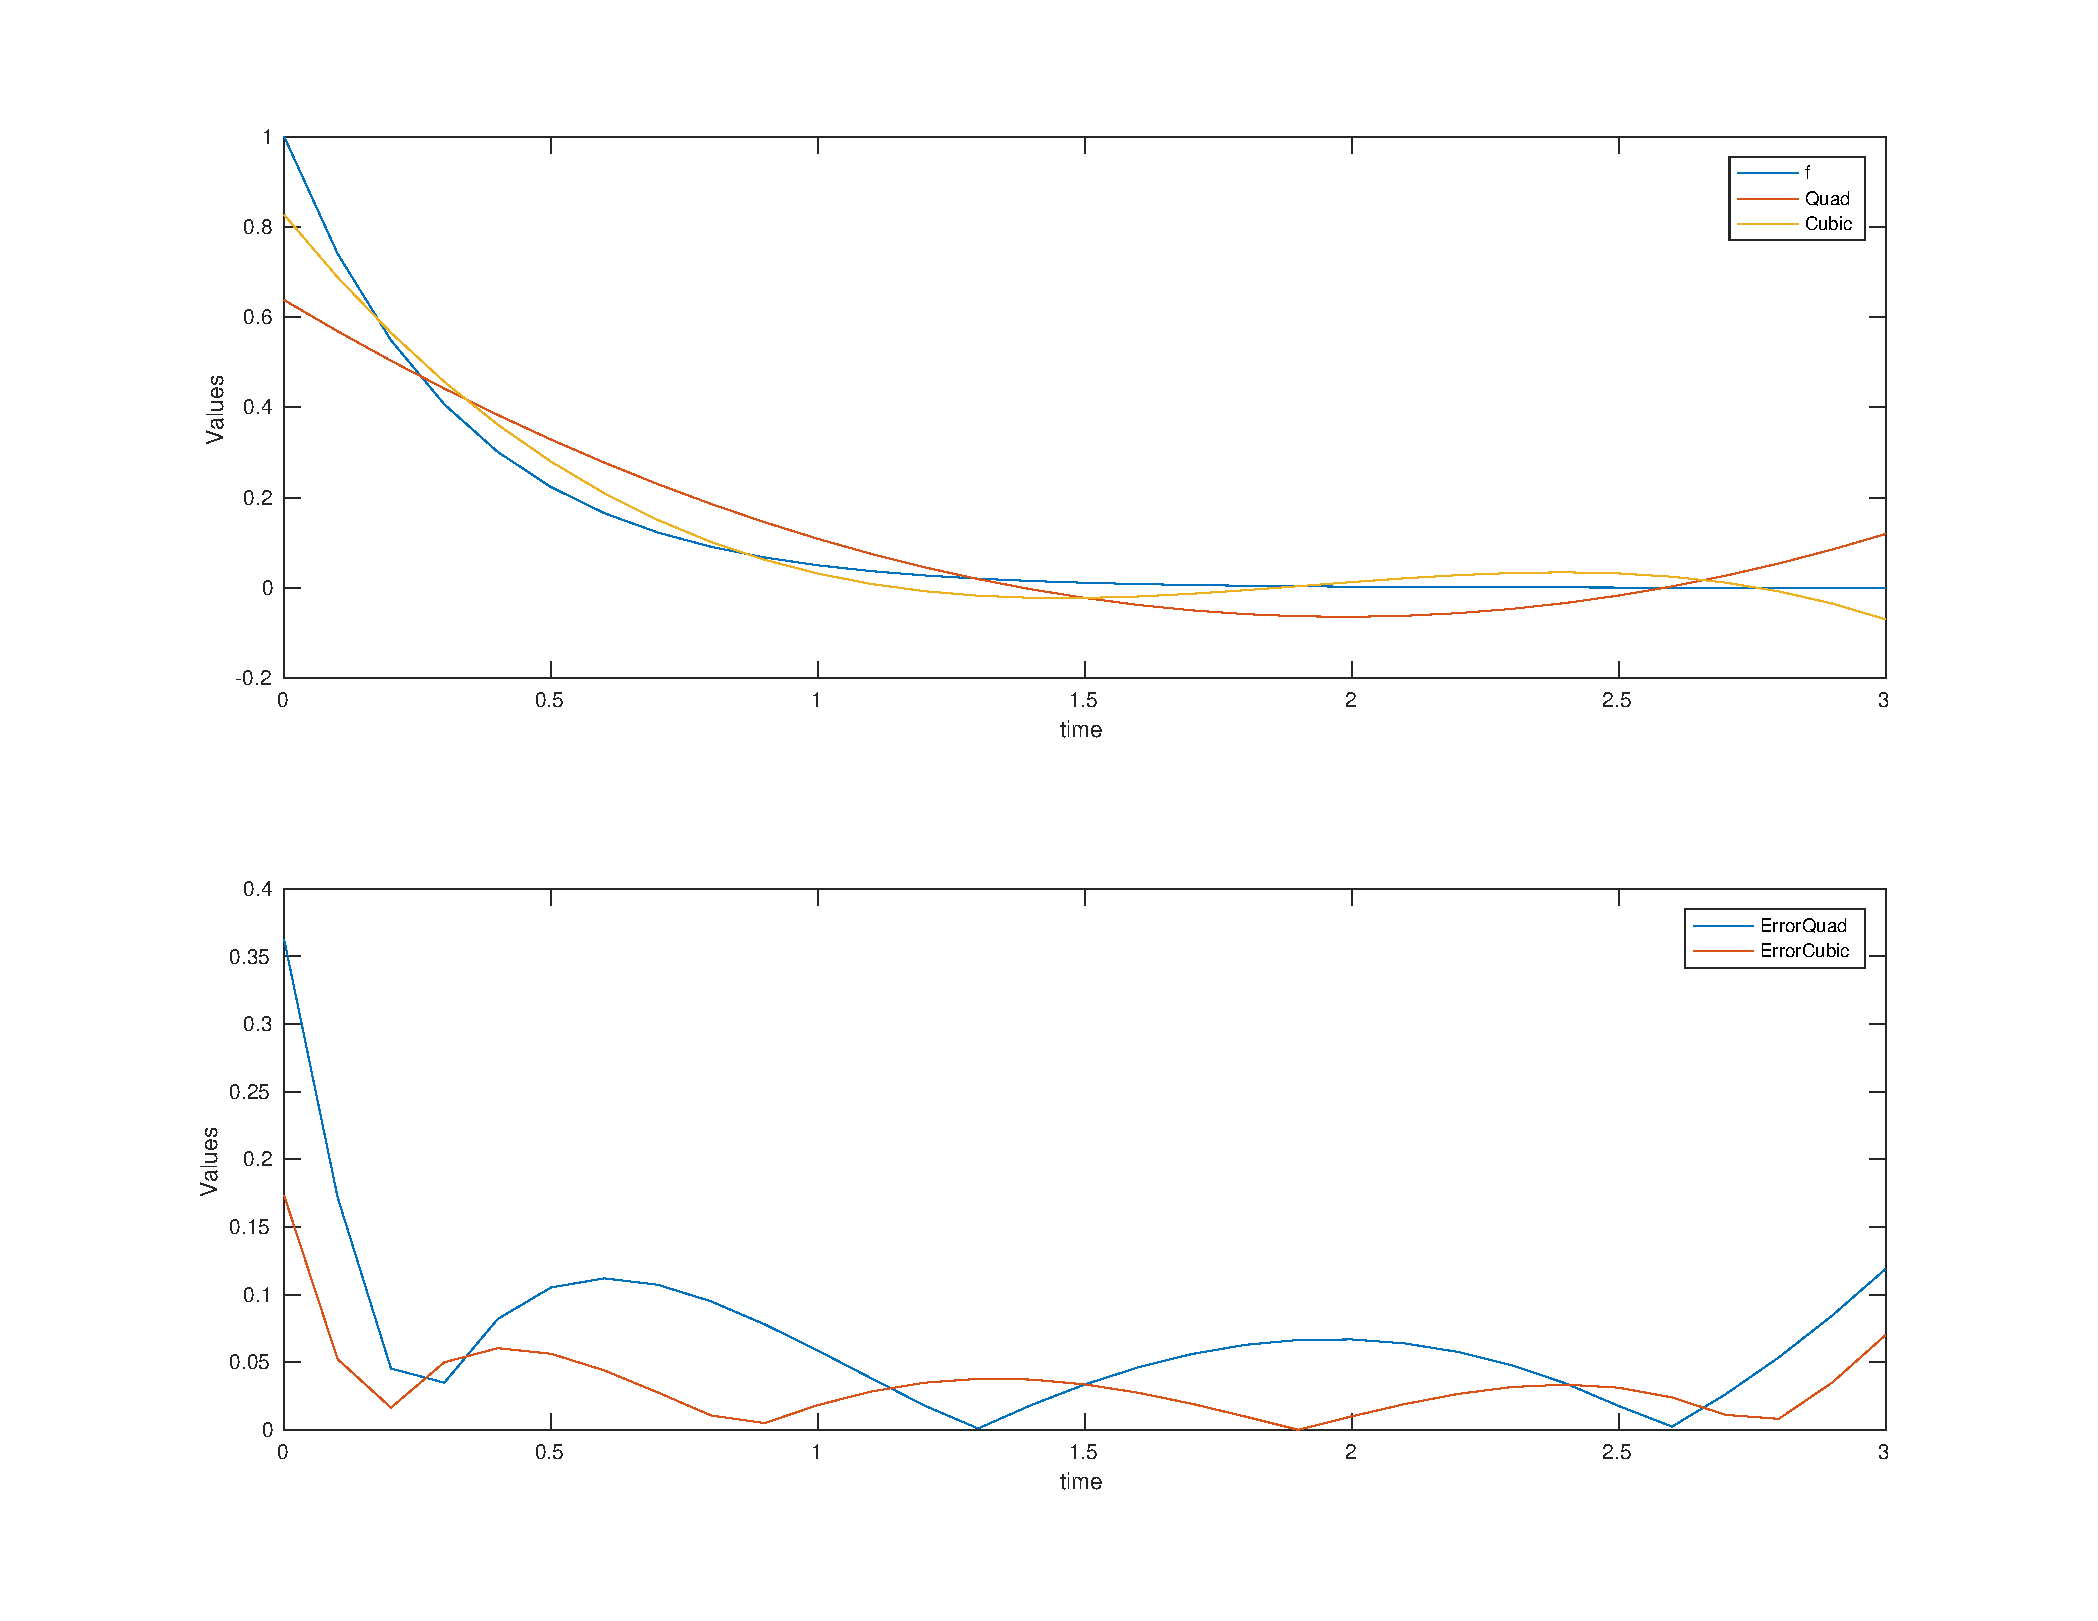
\includegraphics[width=12cm, height=12cm]{Prob1}
  \caption{Quadratic and Cubic Polynomial Approximation}
  \end{figure}

  As the plot shows, the cubic polynomial(yellow line) very closely approximates the original than the quadratic one. The error plot also suggests, that the error magnitude mostly is much higher for the quadratic polynomial than the cubic polynomial. The evaluated l2norm of the error functions, gives \textbf {l2-norm of quad = 0.53115307} and \textbf{l2-norm of cubic = 0.25287738}, indicating that the cubic is a better approximating polynomial in this case. \newline

  \part{c} For orthogonal basis functions, we have $\int_{a}^{b} \phi_j \phi_k = 0, for j\neq k$. Thus, each additional orthogonal basis added to the approximating polynomial aims to reduce the residual from the previous set of basis functions. Since, it always reduces the residue , it cannot make the approximating polynomial any worse than the lower degree polynomial.
  

  \question{Question-2}{Chapter-14, question-2}
  Let f(x) be a given function that can be evaluated at points $x_o \pm jh, j=0,1,2,\dots$ for any fixed value of h, $0 < h << 1$. \newline
  \part{a} Using Taylor series expansion about $x_0$, we can write the following expansions about $\pm h$:
  \[ f(x_0 + h) = f(x_0) + hf^\prime(x_0) + \dfrac{h^2}{2}f^{\prime\prime}(x_0) + \dfrac{h^3}{6}f^{\prime\prime\prime}(x_0) + \dfrac{h^4}{24}f^{\prime\prime\prime\prime}(x_0) + \dfrac{h^5}{120}f^{\prime\prime\prime\prime\prime}(\zeta_1) \]
  \[ f(x_0 - h) = f(x_0) - hf^\prime(x_0) + \dfrac{h^2}{2}f^{\prime\prime}(x_0) - \dfrac{h^3}{6}f^{\prime\prime\prime}(x_0) + \dfrac{h^4}{24}f^{\prime\prime\prime\prime}(x_0) - \dfrac{h^5}{120}f^{\prime\prime\prime\prime\prime}(\zeta_2) \]
  where, $x_0 \leq \zeta_1 \leq x_0 + h$, and $x_0 - h \leq \zeta_2 \leq x_0$
  The difference of the above two equations gives the following:
  \begin{equation}
  f(x_0+h) - f(x_0-h) = 2\{ hf^\prime(x_0) + \dfrac{h^3}{6}f^{\prime\prime\prime}(x_0) + \dfrac{h^5}{120}f^{\prime\prime\prime\prime\prime}(\zeta_3) \}
  \label{eq:1ptdiff}
  \end{equation}
  where, $x_0 - h \leq \zeta_3 \leq x_0 + h$

  Similarly, we can get the following expansions using nearby points at $x_0 \pm 2h$:
  \[ f(x_0 + 2h) = f(x_0) + 2hf^\prime(x_0) + \dfrac{4h^2}{2}f^{\prime\prime}(x_0) + \dfrac{8h^3}{6}f^{\prime\prime\prime}(x_0) + \dfrac{16h^4}{24}f^{\prime\prime\prime\prime}(x_0) + \dfrac{32h^5}{120}f^{\prime\prime\prime\prime\prime}(\zeta_4) \]
  \[ f(x_0 - 2h) = f(x_0) - 2hf^\prime(x_0) + \dfrac{4h^2}{2}f^{\prime\prime}(x_0) - \dfrac{8h^3}{6}f^{\prime\prime\prime}(x_0) + \dfrac{16h^4}{24}f^{\prime\prime\prime\prime}(x_0) - \dfrac{32h^5}{120}f^{\prime\prime\prime\prime\prime}(\zeta_5) \]
  where, $x_0 \leq \zeta_4 \leq x_0 + 2h$, and $x_0 - 2h \leq \zeta_5 \leq x_0$
  The difference of the above two equations gives the following:
  \begin{equation}
  f(x_0+2h) - f(x_0-2h) = 2\{ 2hf^\prime(x_0) + \dfrac{8h^3}{6}f^{\prime\prime\prime}(x_0) + \dfrac{32h^5}{120}f^{\prime\prime\prime\prime\prime}(\zeta_6) \}
  \label{eq:2ptdiff}
  \end{equation}
  where, $x_0 - 2h \leq \zeta_6 \leq x_0 + 2h$

  Then multiplying $\eqref{eq:1ptdiff}$ by 2 and subtracting it from $\eqref{eq:2ptdiff}$, we get:
  \[ f(x_0 + 2h) - f(x_0 - 2h) - 2f(x_0 + h) + 2f(x_0-h) = 2h^3f^{\prime\prime\prime}(x_0) + \dfrac{h^5}{2}f^{\prime\prime\prime\prime\prime}(\zeta) \]
  where, $z_0 - 2h \leq \zeta \leq x_0 + 2h$
  Rearranging the terms, we get:
  \begin{equation}
	  f^{\prime\prime\prime}(x_0) = \dfrac{f(x_0 + 2h) - f(x_0 - 2h) - 2f(x_0 + h) + 2f(x_0-h)}{2h^3} + \mathbf{\dfrac{-h^2}{4}f^{\prime\prime\prime\prime\prime}(\zeta)}
	  \label{eq:3deriv}
  \end{equation}

  $\eqref{eq:3deriv}$ provides the formula for approximating the third derivative $f^{\prime\prime\prime}(x_0)$, with the bold test showing the component of the truncation error:
  Thus, truncation error = $\mathbf{\dfrac{-h^2}{4}f^{\prime\prime\prime\prime\prime}(\zeta)}$

  \part{d} The below figure shows the plot of the approximated 3rd derivative derived as above.
  \begin{figure}[H]
   \centering
  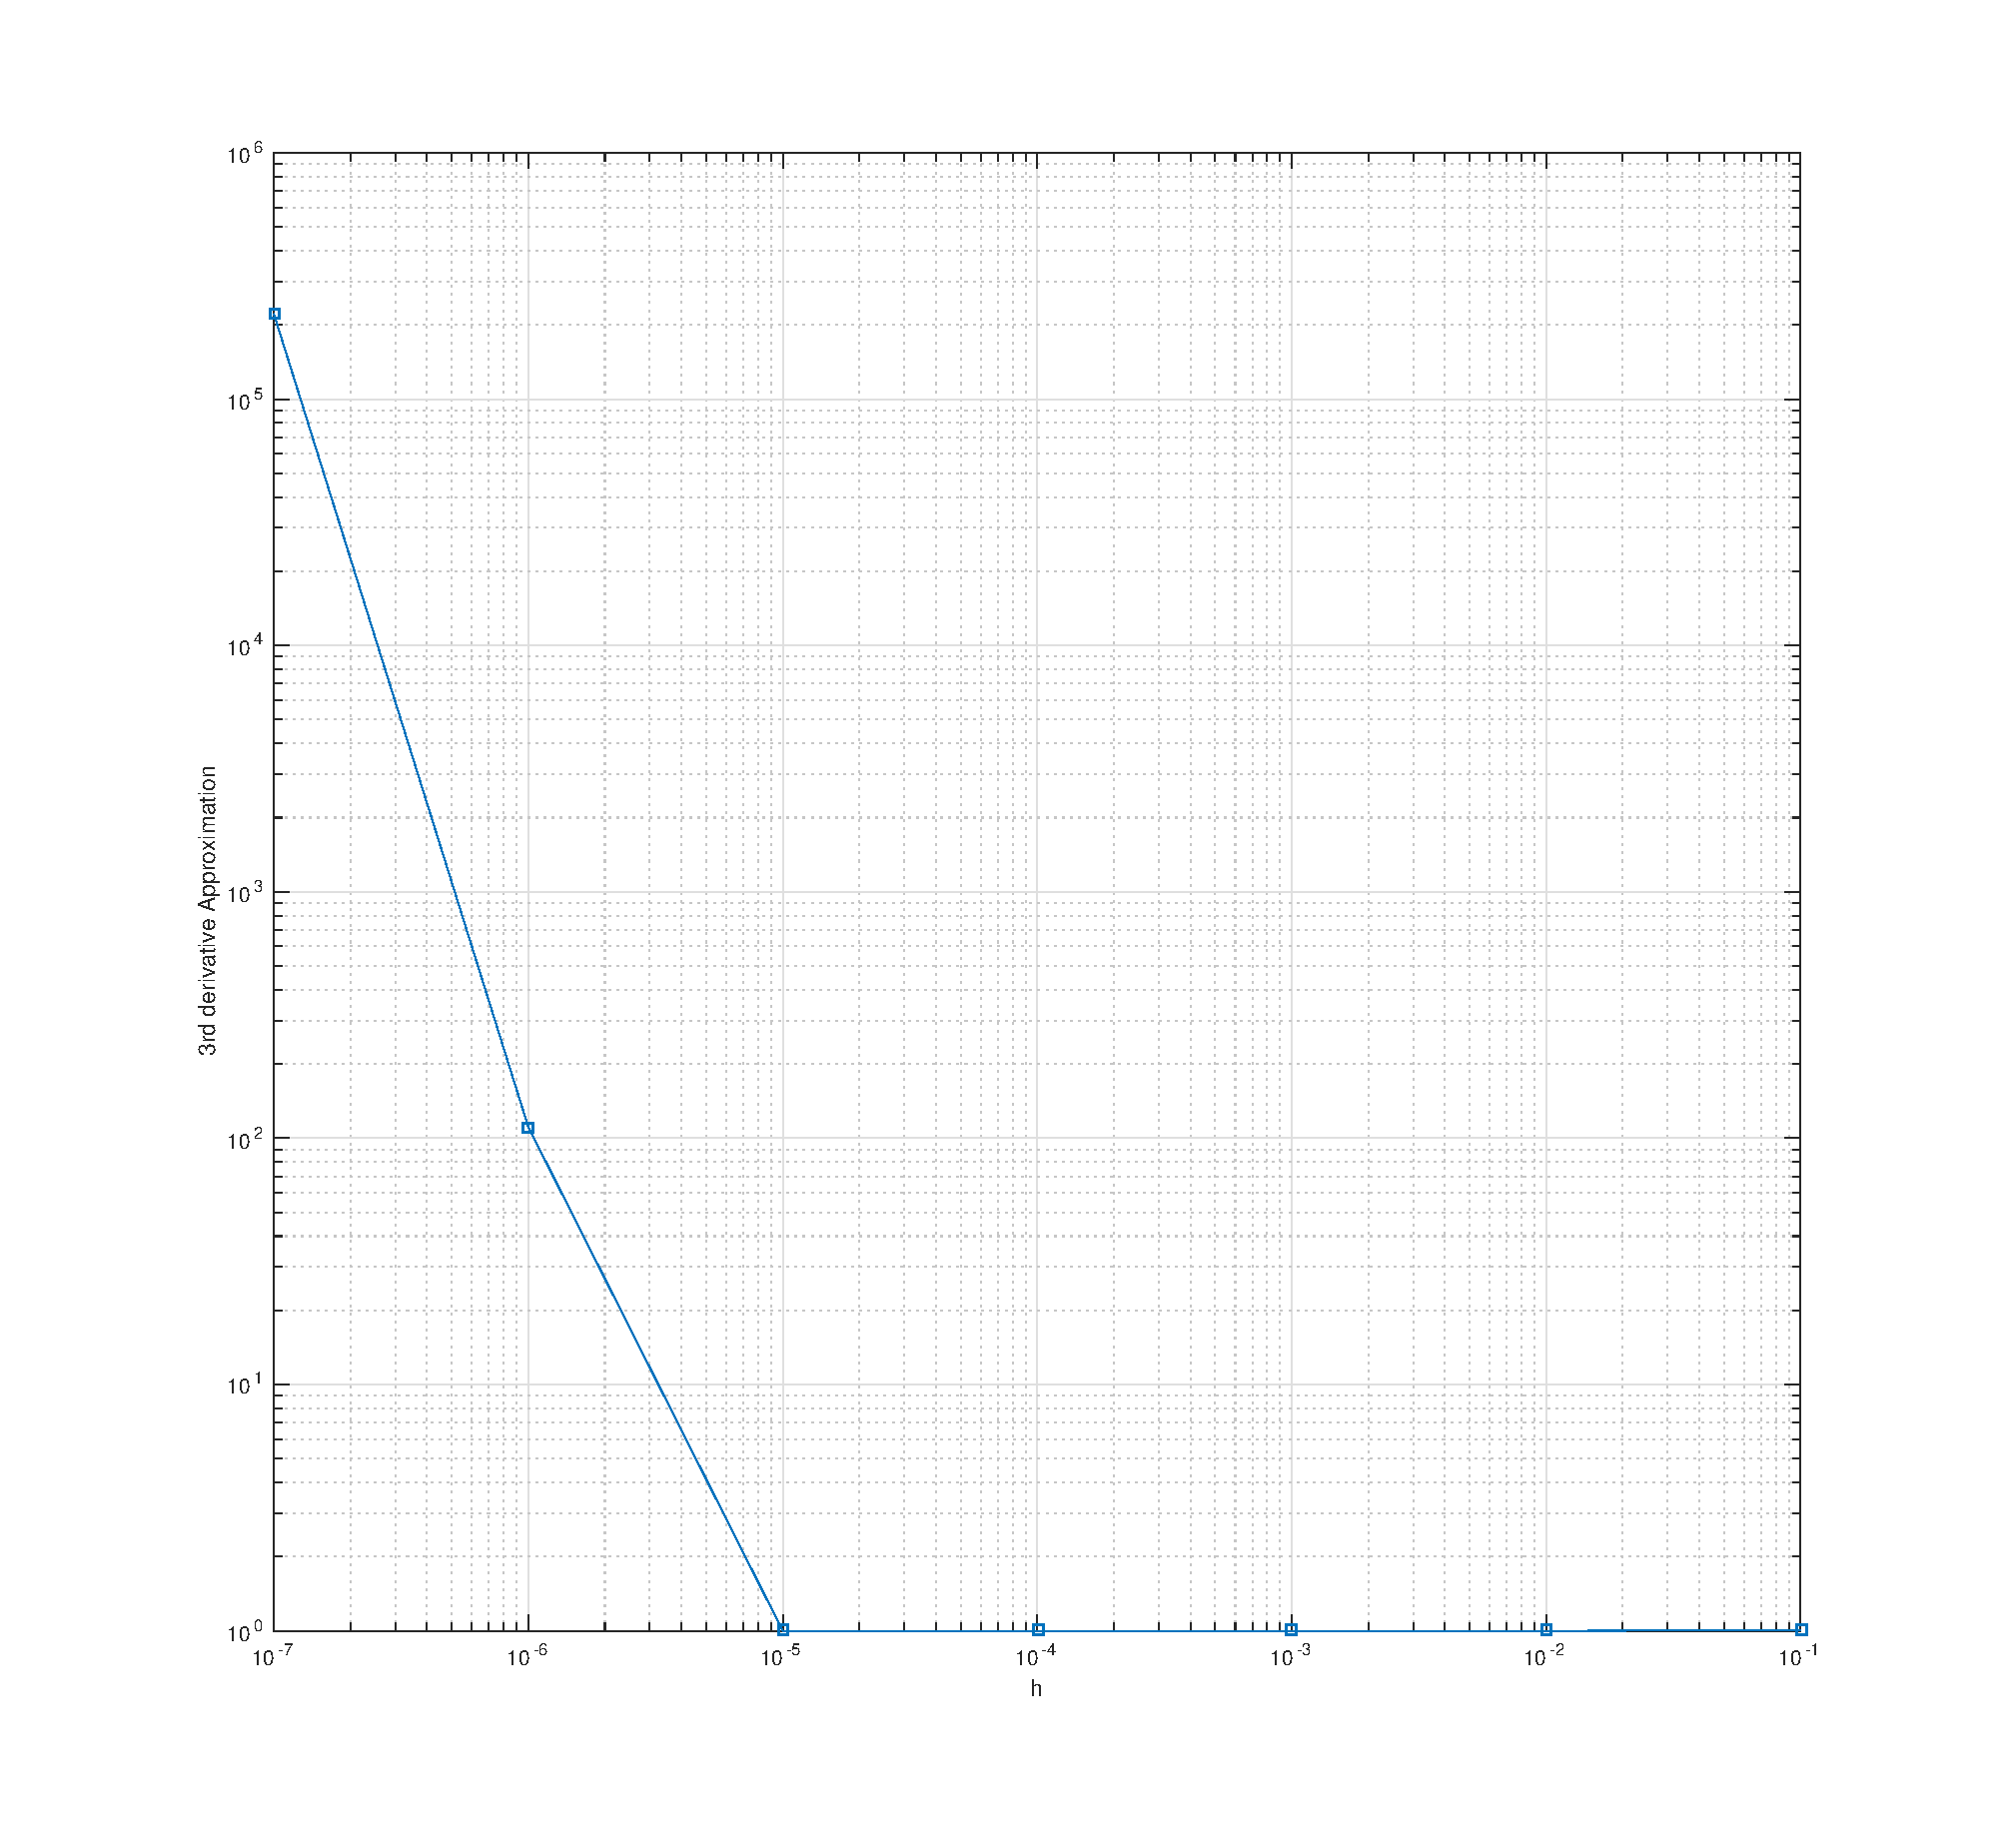
\includegraphics[width=12cm, height=12cm]{Prob2}
  \caption{Approximated 3rd derivative}
  \end{figure}
  
  As the figure suggests, beyond $h=10^{-5}$, the round-off error dominates. Since the true value of the function is 1 at $x=0$, hence the deviation of the curve from the x-axis depicts the magnitude iof the error due to increasing round-off with reducing values of h. However, for larger values of h, it is quite accurate. We plot an expanded plot in the range where it shows high accuracy as below:
  \begin{figure}[H]
   \centering
  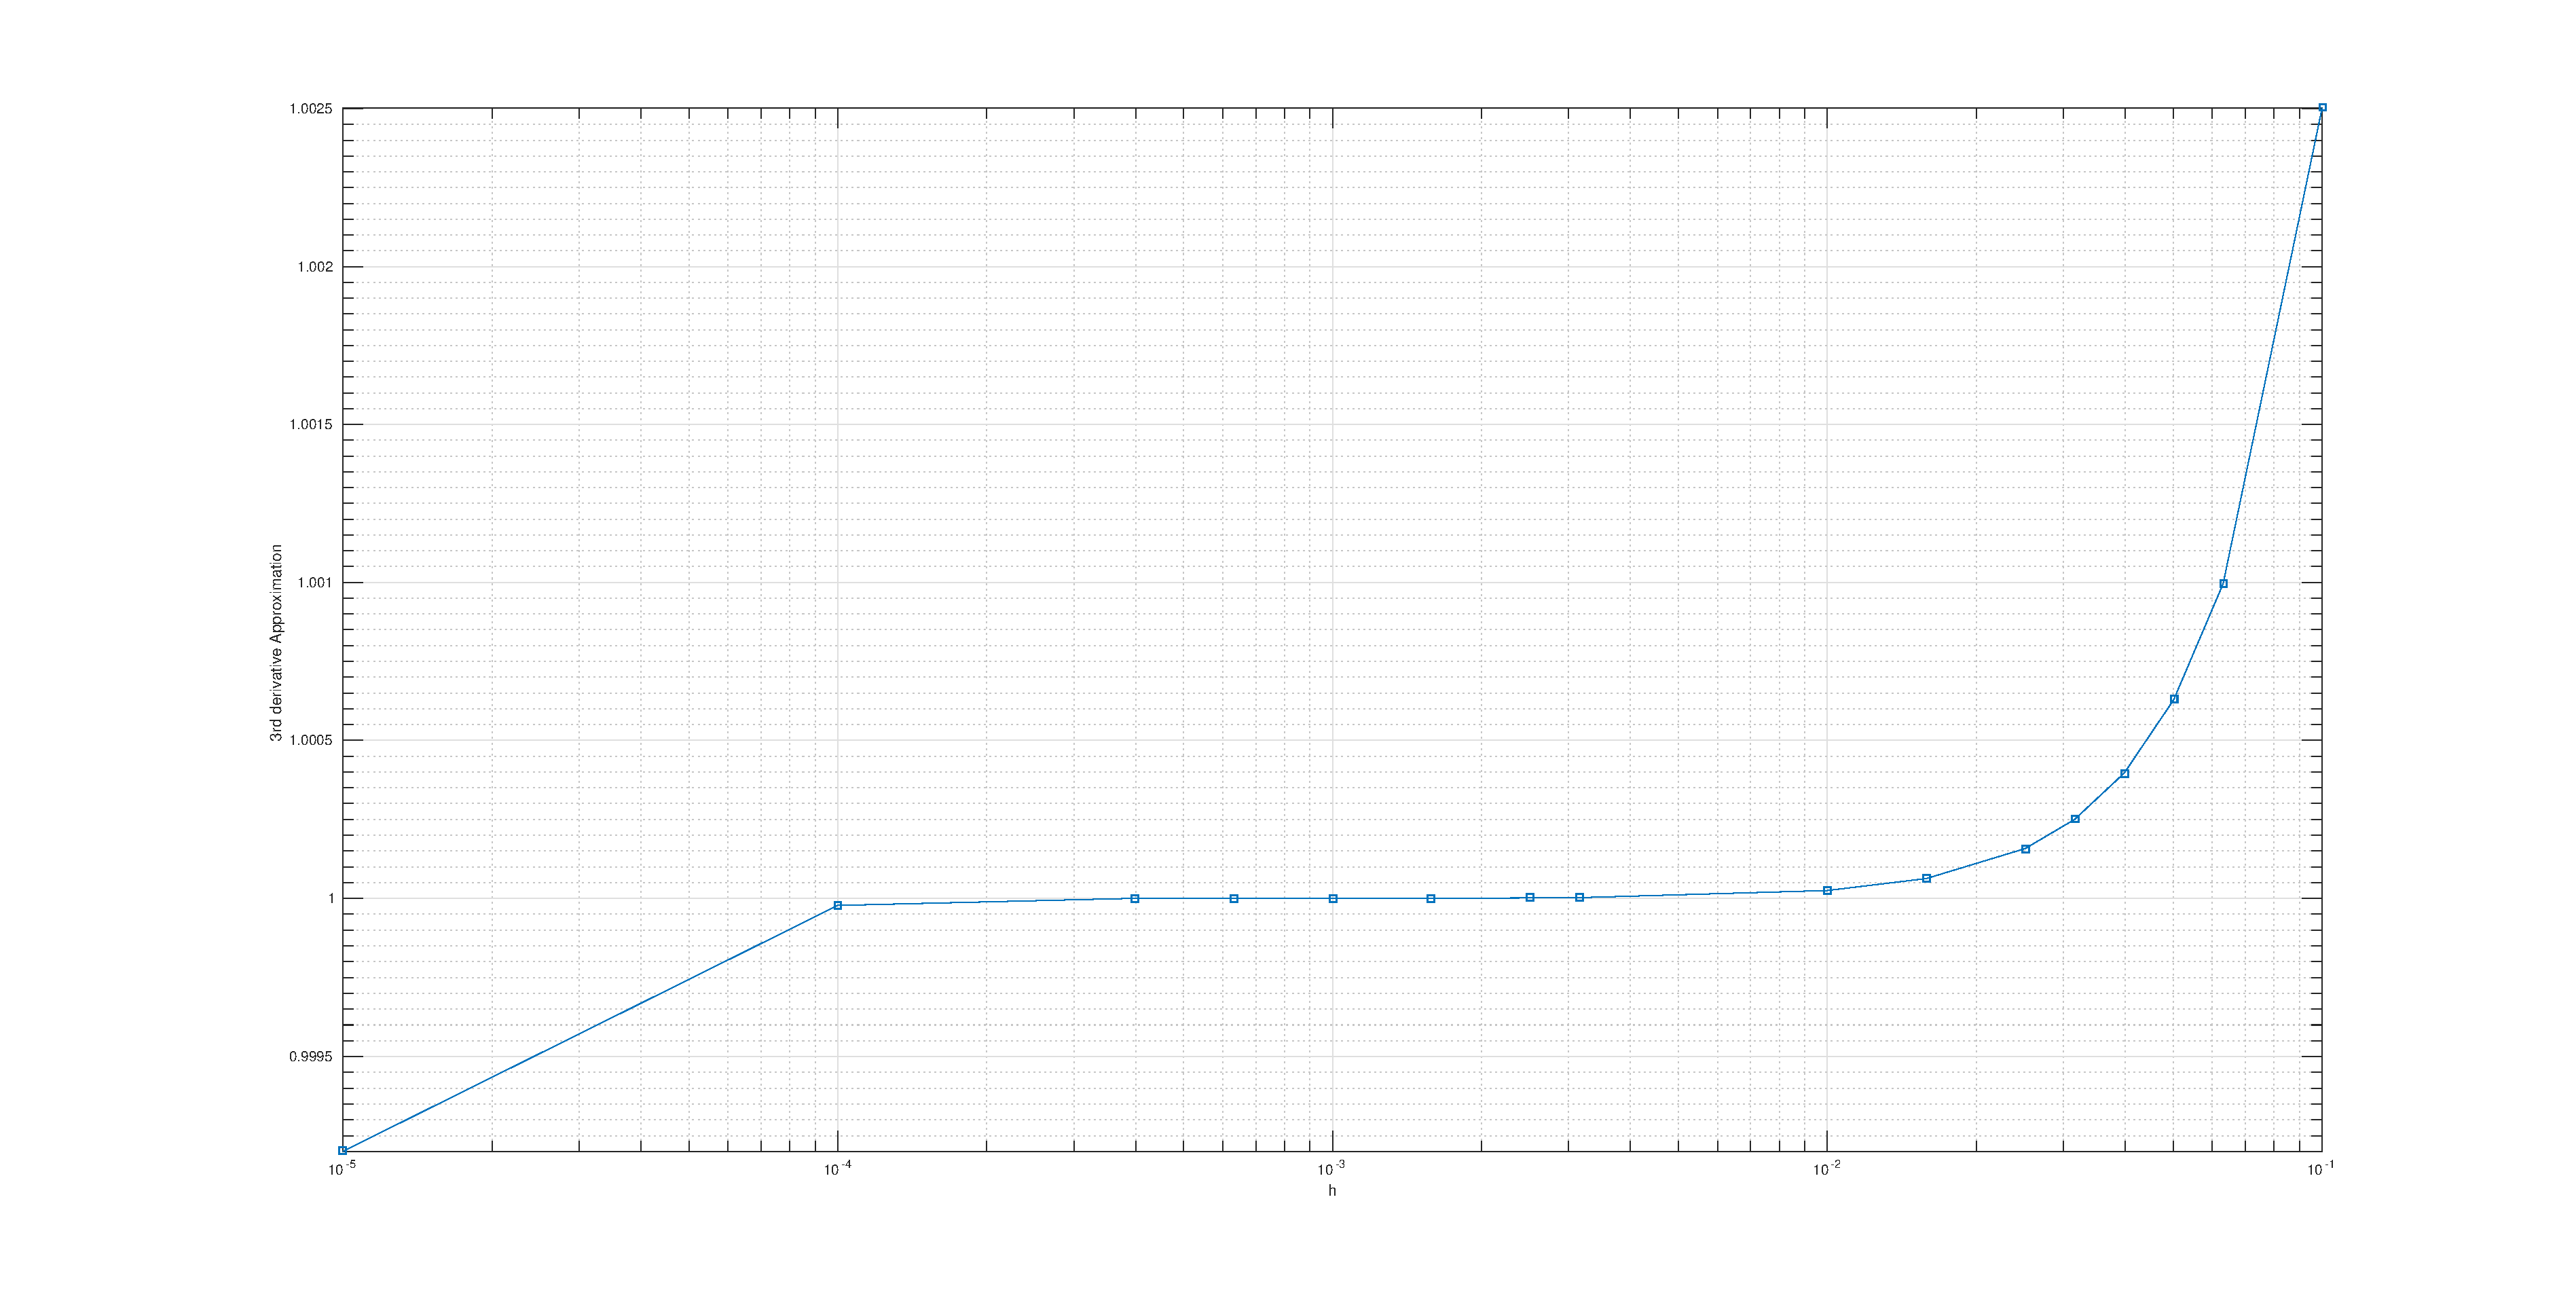
\includegraphics[width=12cm, height=12cm]{Prob2_quad}
  \caption{Improved accuracy at higher h}
  \end{figure}

  As the parabolic shape of the curve suggests that the approximation is indeed second order accurate for large values of h. Best value of approximation we get for $h \approx 10^{-3}$. \newline


  \part{c} To derive the expression for the round-off error, we denote the floating point evaluations of $f$ by $F$. Thus the expression for round off error will be $|F^{\prime\prime\prime}(x_0) - f^{\prime\prime\prime}(x_0)|$ \[ = \bigg |  \dfrac{F(x_0 + 2h) - F(x_0 - 2h) - 2F(x_0 + h) + 2F(x_0-h)}{2h^3} - \dfrac{f(x_0 + 2h) - f(x_0 - 2h) - 2f(x_0 + h) + 2f(x_0-h)}{2h^3} \bigg |\]
  \[= \bigg |  \dfrac{e_r(x_0+2h) - e_r(x_0-2h) -2e_r(x_0+h) + 2e_r(x_0-h)}{2h^3}  \bigg |\]
  where, the round-off error term, $e_r(x) = F(x) - f(x)$
  \[\leq \bigg | \dfrac{e_r(x_0 + 2h)}{2h^3}\bigg | + \bigg | \dfrac{e_r(x_0 - 2h)}{2h^3}\bigg | + \bigg | \dfrac{2e_r(x_0 + h)}{2h^3}\bigg | + \bigg | \dfrac{2e_r(x_0 - h)}{2h^3}\bigg |\]
  Assuming the each round-off error term is bounded by the machine precision, $\epsilon$, then we get:
  \[ |F^{\prime\prime\prime}(x_0) - f^{\prime\prime\prime}(x_0)| \leq \dfrac{6\epsilon}{2h^3} = \dfrac{3\epsilon}{h^3} \]

  Thus, the round-off error grows inversely proportional to $h$. Hence, as h decreases, the round-off error increases, thus with $h->0$, the round-off error will tend to $\infty$ .

  \part{d} We can obtain a fourth order formula in a similar manner as we obtained the third order formula with some minor changes. First evaluate $S1: f(x_0 + h) + f(x_0 - h)$, then evaluate $S2: f(x_0 + 2h) + f(x_0 - 2h)$. Then subtract $S2 - 4S1$, to extract the fourth order formula.

  \question{Question-3}{Chapter-14: question-8}
  Derivation of an approximate formulae for the second derivatives $f^{\prime\prime}(x_0)$ of a smooth function $f(x)$ using the three points $x_{-1},x_0 = x_{-1} + h_0, x_1=x_0 + h_1$, where $h_0 \neq h_1$. 

  \part{a} To prove both the given approximations are the same, we need to show: $2[f_{x-1,x_0,x_1}] = \dfrac{g_{1/2} - g_{-1/2}}{(h_0+h_1)/2}$. \newline
  \textbf {Proof:} \newline
  Using divided difference, we can write:
  \[2[f_{x-1,x_0,x_1}] = 2 \times \dfrac{\dfrac{f(x_1)-f(x_0)}{x_1 - x_0}-\dfrac{f(x_0) - f(x_{-1})}{x_0 - x_{-1}}}{x_1 - x_{-1}}\]
  \[2[f_{x-1,x_0,x_1}] = 2 \times \dfrac{\dfrac{f(x_1)-f(x_0)}{h_1}-\dfrac{f(x_0) - f(x_{-1})}{h_0}}{h_1 + h_0}\]
  Given, that: $g_{1/2} = \dfrac{f(x_1)-f(x_0)}{h_1}$ and $g_{-1/2} = \dfrac{f(x_0) - f(x_{-1})}{h_0},$ we can replace them to get:
  \[2[f_{x-1,x_0,x_1}] = 2 \times \dfrac{g_{1/2}-g_{-1/2}}{h_1 + h_0}\]
  \[2[f_{x-1,x_0,x_1}] = \dfrac{g_{1/2}-g_{-1/2}}{\dfrac{h_1 + h_0}{2}}\]

  \part{b} To show that the method is only first order accurate, we use the Taylor series expansion upto second order with third order error term to derive the formualation:\newline
  \[f(x_0 + h_1) = f(x_0) + h_1f^\prime(x_0) + \dfrac{h_1^2}{2}f^{\prime\prime}(x_0) + \dfrac{h_1^3}{3!}f^{\prime\prime\prime}(\zeta_1)\]
  \[f(x_0 - h_0) = f(x_0) - h_0f^\prime(x_0) + \dfrac{h_0^2}{2}f^{\prime\prime}(x_0) - \dfrac{h_0^3}{3!}f^{\prime\prime\prime}(\zeta_2)\]
  Which can be further simplified to:
  \[\dfrac{f(x_1) - f(x_0)}{h_1} =  f^\prime(x_0) + \dfrac{h_1}{2}f^{\prime\prime}(x_0) + \dfrac{h_1^2}{3!}f^{\prime\prime\prime}(\zeta_1)\]
  \[\dfrac{f(x_{-1}) - f(x_0)}{h_0} = -f^\prime(x_0) + \dfrac{h_0}{2}f^{\prime\prime}(x_0) - \dfrac{h_0^2}{3!}f^{\prime\prime\prime}(\zeta_2)\]

  Adding these two, we get:
  \[\dfrac{f(x_1) - f(x_0)}{h_1} - \dfrac{f(x_{0}) - f(x_{-1})}{h_0} = \dfrac{(h_0 + h_1)}{2}f^{\prime\prime}(x_0) + \dfrac{h_1^2}{3!}f^{\prime\prime\prime}(\zeta_1) - \dfrac{h_0^2}{3!}f^{\prime\prime\prime}(\zeta_2)\]

  For the error term, replacing with a $\zeta$, such that $x_{-1} \leq \zeta \leq x_1$:
  \[\dfrac{f(x_1) - f(x_0)}{h_1} - \dfrac{f(x_{0}) - f(x_{-1})}{h_0} = \dfrac{(h_0 + h_1)}{2}f^{\prime\prime}(x_0) + f^{\prime\prime\prime}(\zeta)(\dfrac{h_1^2}{3!} - \dfrac{h_0^2}{3!})\]

  Rearranging to get the second order term:
  \[f^{\prime\prime}(x_0) = \dfrac{\dfrac{f(x_1) - f(x_0)}{h_1} - \dfrac{f(x_{0}) - f(x_{-1})}{h_0}}{(h_0 + h_1)/2} - \mathbf{\dfrac{f^{\prime\prime\prime}(\zeta)(h_1 - h_0)}{3}}\]

  The error term shown in bold is thus only first order,$O(h_0 + h_1)$ , accurate.

  

  \part{c} The matlab code file is $Prob3.m$, where we run the two methods above for second derivative approximation of first order accuracy for the given values of h, around the point $x_0 = 0$. Both methods do not show any deviation from each other, that is, their mutual difference is zero.
  Thus, the table will be :
  \begin{longtable}{c|c|c|c}
	\caption{Second derivative approximation result for $e^x$ at $x=0$} \\
  %\centering
  %\begin{tabular}{c c c c}
  \hline\hline
	  h & firstMethod & secondMethod & difference \\ [0.5ex]
	  1.0e-1 & 14.0227 &  14.0227 & 0 \\
	  1.0e-2 & 134.00 &   134.00 & 0 \\
	  1.0e-3 & -1334.00 & -1334.00 & 0 \\
	  1.0e-4 & 13334.00 & 13334.00 & 0 \\
	  1.0e-5 & 133334.00 & 133334.00 & 0  \\
  \hline

  \end{longtable}

	  The results are extremely inaccurate for an approximation of second order derivative of $e^x$ at $x=0$. This happens mainly because of round-off as we keep reducing h. Since, there are subtracting terms of very lose values, round-off  escalates the error to large values.

  \begin{longtable}{c|c|c|c}
	\caption{Second derivative approximation result for $sinx$ at $x=1.2$} \\
  %\centering
  %\begin{tabular}{c c c c}
  \hline\hline
	  h & firstMethod & secondMethod & difference \\ [0.5ex]
  
$10^{0}$ & 0.075126648647425 & 0.075126648647425 & 0 \\
$10^{-0.5}$ & 0.007741148589218 & 0.007741148589218 & 0 \\
$10^{-1.0}$ & 0.000776440384795 & 0.000776440384795 & 0.000000222044605 \\
$10^{-1.5}$ & 0.000077667334949 & 0.000077667334949 & 0.000000777156117 \\
$10^{-2.0}$ & 0.000007766966345 & 0.000007766966345 & 0                 \\
$10^{-2.5}$ & 0.000000776702422 & 0.000000776702429 & 0.000006661338148 \\
$10^{-3.0}$ & 0.000000077772619 & 0.000000077772619 & 0                 \\
$10^{-3.5}$ & 0.000000008938792 & 0.000000008938954 & 0.000162203583898 \\
$10^{-4.0}$ & 0.000000006718345 & 0.000000006718345 & 0                 \\
$10^{-4.5}$ & 0.000000084433957 & 0.000000084433986 & 0.000028532731733 \\
$10^{-5.0}$ & 0.000001305679284 & 0.000001305679284 & 0.000000111022302 \\
$10^{-5.5}$ & 0.000006856794407 & 0.000006856780840 & 0.013567702517037 \\
$10^{-6.0}$ & 0.000117879096870 & 0.000117879096870 & 0                 \\
$10^{-6.5}$ & 0.001672191331345 & 0.001672191233429 & 0.097916452723723 \\
$10^{-7.0}$ & 0.010553975528346 & 0.010553975528346 & 0.000000111022302 \\
$10^{-7.5}$ & 0.154882968729617 & 0.154882969473164 & 0.743547445836157 \\
	  $10^{-8.0}$ & 0.932039085967226 & 0.932039085967226 & 0 \\ [1ex]
	  
	  
	  
	  
	  
	  
	  
	  
	  
	  
	  
	  
	  
	  
   \hline

  \end{longtable}
	  
  

  \question{Question-4}{Chapter-14, question-13}
  \part{b} Here we denote the two methods as:\newline
	  \textbf{First Method:} $(f_1 - 2f_0 + f_1)/h^2$ \newline
	  \textbf{Second Method:} $\dfrac{g_{1/2} - g_{-1/2}}{h}$, where $g_{1/2} = \dfrac{f_1 - f_0}{h}$ and $g_{-1/2} = \dfrac{f_0 - f_{-1}}{h}$.

	  The below table reports the error/deviations of these methods from the true second order derivative for $f(x)=sin(x)$ at $x0=1.2$

  \question{Question-5}{Chapter-14, question-15}
  Consider the numerical differentiation of the function, $f(x) = c(x)e^{x/\pi}$, defined on $[0,\pi]$, where
  \[c(x) = j; \dfrac{\pi}{4}(j-1) \leq x < \dfrac{\pi}{4}j\]
  for $j=1,2,3,4,\dots$
  \part{a} We want a difference approximation with step size, $h = \dfrac{n}{\pi}$. Suppose, we have n as multiple of 4, that is, $n=4l$, where $l$ is an integer. Since, the points are equispaced, thus the entire $[0,\pi]$ region can be seen as partioned into 4 regions each having $l$ points as described below: \newline
  $\mathbf {L1:} 0 \leq x < \pi/4$ : $l$ points at $0, \dfrac{\pi}{4l}, \dfrac{2\pi}{4l}, \dots, \dfrac{(l-1)\pi}{4l}$ \newline
  $\mathbf {L2:} \pi/4 \leq x < \pi/2$ : $l$ points at $\dfrac{\pi}{4}, \dfrac{\pi}{4} + \dfrac{\pi}{4l},\dfrac{\pi}{4} + \dfrac{2\pi}{4l}, \dots, \dfrac{\pi}{4} + \dfrac{(l-1)\pi}{4l}$ \newline
  $\mathbf {L3:} \pi/2 \leq x < 3\pi/4$ : $l$ points at $\dfrac{\pi}{2}, \dfrac{\pi}{2} + \dfrac{\pi}{4l},\dfrac{\pi}{2} + \dfrac{2\pi}{4l}, \dots, \dfrac{\pi}{2} + \dfrac{(l-1)\pi}{4l}$ \newline
  $\mathbf {L4:} 3\pi/4 \leq x < \pi$ : $l$ points at $\dfrac{3\pi}{4}, \dfrac{3\pi}{4} + \dfrac{\pi}{4l},\dfrac{3\pi}{4} + \dfrac{2\pi}{4l}, \dots, \dfrac{3\pi}{4} + \dfrac{(l-1)\pi}{4l}$ \newline
  The last point is at $\pi$ \newline
  Now, $c(x)$ is discontinuous at the points of integer multiples of $\pi/4$. To make sure that the discontinuities do not affect out difference formulation it is beneficial to have some of the interval end points at these discontinuities. For example, if we want to approximate the difference value at a point $t$ in the interval $[x_{i-1}, x_i]$, there will be two possibilities while taking the difference. If $x_{i-1}$ and $x_{i}$ lie in the same region described above, then $c(x)$ has the same values at both the points and can be approximated with the value of $c(x_{i-1})$. If on the other hand, $x_{i-1}$ and $x_i$ lie in two different regions, the only possibility is the $x_{i-1}$ is the last point in one region while $x_i$ is the first point of the other region and hence we have a discontinuity at $x_i$ , however, $t$ will be in the region of $x_{i-1}$ and hence to avoid the discontinuity in the calculation, we can take the left continuous value at $x_i$, which will be equal to the value at $t_i$. Hence, with n being multiple of 4, we have the possibility of avoiding the discontinuities resulting in better values. Consider on the other hand, if n was not a multiple of 4, that is, we did not had this nice region partition, then the point $t$ could itself have a discontinuity which we could not be able to derive from the sampling points $[x_{i-1},x_i]$. Moreoever, suppose we have $t$ in $[x_{i-1},x_i]$, where $c(x_{i-1}) \neq c(x)$, and t lies not at the point of discontinuity, but either in the step with $x_{i-1}$ or with $x_i$. All these points lying on either side of the step, will get the same difference value which will be highly inaccurate. These issues we can solve by having n has multiple of 4, and having the nice partitioning described above . \newline

  \part{b}\textbf {Show that:} $h^{-1}c(t_i)(e^{x_{i+1}/\pi} - e^{x_i/\pi})$ provides a second order approximation of $f^\prime(t_i)$ \newline
  \textbf{Proof:} $t_i = x_i + \dfrac{h}{2} = ih + \dfrac{h}{2} = (i + \dfrac{1}{2})h$; $i=0,1,\dots,(n-1)$ \newline
  Using Taylor series expansion around the point $t_i = x_i + \dfrac{h}{2}$, we can write:'
  \[f(x_i + \dfrac{h}{2} - \dfrac{h}{2}) = f(x_i + \dfrac{h}{2}) - \dfrac{h}{2}f^\prime(x_i + \dfrac{h}{2}) + \dfrac{h^2}{4}f^{\prime\prime}(x_i + \dfrac{h}{2}) - \dfrac{h^3}{8}f^{\prime\prime\prime}(\zeta_1)\]
  and, 
  \[f(x_i + \dfrac{h}{2} + \dfrac{h}{2}) = f(x_i + \dfrac{h}{2}) + \dfrac{h}{2}f^\prime(x_i + \dfrac{h}{2}) + \dfrac{h^2}{4}f^{\prime\prime}(x_i + \dfrac{h}{2}) + \dfrac{h^3}{8}f^{\prime\prime\prime}(\zeta_2)\]
  Subtracting $f(x_{i+1}=x_i+h) - f(x_{i})$ gives, 
  \[ f(x_{i+1}) - f(x_i) = hf^\prime(x_i + \dfrac{h}{2}) + \dfrac{h^3}{8}\{ f^{\prime\prime\prime}(\zeta_1) + f^{\prime\prime\prime}(\zeta_2)\} \]
  where $t_i - h/2 \leq \zeta_1 \leq t_i$ and $t_i \leq \zeta_2 \leq t_i + h/2$. Choosing a $\zeta$, such that, $t_i - h/2 \leq \zeta \leq t_i + h/2$, we can then write:
  \[ f(x_{i+1}) - f(x_i) = hf^\prime(x_i + \dfrac{h}{2}) + \dfrac{h^3}{4}\{ f^{\prime\prime\prime}(\zeta)\} \]
  Since, $t_i = x_i + h/2$,
  \[ f(x_{i+1}) - f(x_i) = hf^\prime(t_i) + \dfrac{h^3}{4}\{ f^{\prime\prime\prime}(\zeta)\} \]
  \[ f^\prime(t_i) = \dfrac{f(x_{i+1}) - f(x_i)}{h} - \dfrac{h^2}{4}f^{\prime\prime\prime}(\zeta)\]
  \[ f^\prime(t_i) = \dfrac{c(x_{i+1})e^{x_{i+1}/\pi} - c(x_i)e^{x_i/\pi}}{h} - \dfrac{h^2}{4}f^{\prime\prime\prime}(\zeta)\]

  As, described in first part of this question, if the end-points of the interval$[x_i,x_{i+1}]$, $t_i$ belongs to falls completely in one of the regions, then we have $c(x_i) = c(t_i) = c(x_{i+1})$. If $x_i$ and $x_{i+1}$ fall in different region, then $x_{i+1}$ falls in the point of discontinuity, so we take the left continuous value at $x_{i+1}$ which will be equal to $c(t_i) = c(x_i)$. Thus, in the above expression we can replace $c(x_i),c(x_{i+1})$ with $c(t_i)$. Thus we get the following expression:
  \[ f^\prime(t_i) = \dfrac{c(t_i)e^{x_{i+1}/\pi} - c(t_i)e^{x_i/\pi}}{h} - \dfrac{h^2}{4}f^{\prime\prime\prime}(\zeta)\]
  \begin{equation}
   f^\prime(t_i) = \dfrac{c(t_i)(e^{x_{i+1}/\pi} - e^{x_i/\pi})}{h} - \mathbf{\dfrac{h^2}{4}f^{\prime\prime\prime}(\zeta)}
   \label{eq:discont}
  \end{equation}

  $\eqref{eq:discont}$ shows the second order approximantion of $f^\prime(t_i)$



  

  \question{Question-6}{Chapter-15, question-4}
  \part{a} \textbf {Prove:} Error in basic corrected trapezoidal rule in the interval [a,b] can be estimated by:
  \[E(f) = \dfrac{f^{\prime\prime\prime\prime}*(\eta)}{720} (b-a)^5\]
  \textbf {Proof:} The osculating polynomial formula for the basic corrected trapezoidal rule is written as:
  \[p_3(x) = f(a) + f^\prime(a)(x-a) + f[a,a,b](x-a)^2 + f[a,a,b,b](x-a)^2(x-b)\]

  The error in the polynomial interpolation in that case will be fiven by:
  \[f[a,a,b,b,x](x-a)(x-a)(x-b)(x-b)\]

  Then, to find the error in the intergral of the polynomial, we can integrate the error of polynomial described above, in the interval [a,b]
  \[E(f) = \int_{a}^{b} f[a,a,b,b,x]\psi(x)\]
  where $\psi(x) = \prod_{i=0}^{i=3}(x - x_i) = (x-a)(x-a)(x-b)(x-b)$ \newline
  Notice that, since $x$ lies in the interval [a,b], hence $(x-a \geq 0) and (x-b \leq 0)$. In any case, the square of the terms will be greater than equal to 0. So, in the given interval $\psi(x) \geq 0$ always. Because $\psi(x)$ does not changes sign in the interval, then using the intermediate value theorem, there exists $a \leq \eta \leq b$, such that:
  \[E(f) = \int_{a}^{b} f[a,a,b,b,x]\psi(x) = \int_{a}^{b} f[a,a,b,b,\eta]\psi(x)\]
  where,
  \[f[a,a,b,b,\eta] = \dfrac{f^{\prime\prime\prime\prime}(\eta)}{4!}\]
  which is a constant, say $K$. \newline
  Then we can write the error integral as:
  \[E(f) = K \int_{a}^{b} (x-a)^2(x-b)^2 \]
  Doing integration by parts:
  \[E(f) = K\bigg [ \dfrac{(x-a)^2(x-b)^3}{3} - \dfrac{(x-a)(x-b)^4}{6} + \dfrac{(x - b)^5}{30}    \bigg ]_{a}^{b} = \dfrac{-(a-b)^5}{30}\]
  Replacing back K,we get:
  \[E(f) = \dfrac{f^{\prime\prime\prime\prime}(\eta)}{4!}\dfrac{(-(a-b)^5)}{30} = \dfrac{f^{\prime\prime\prime\prime}(\eta)(b-a)^5}{720} \]

  \part{b} The integral for the corrected trapezoidal is written is:
  \[ I_f \approx \int_{a}^{b} p_3(x)dx = \dfrac{(b-a)}{2}[f(a) + f(b)] + \dfrac{(b-a)^2}{12}[f^\prime(a) - f^\prime(b)] \]

  \textbf {part-1:}For the integral $\int_{0}^{1}e^x dx$, thus $a=0,b=1$, and $f(x) = e^x$, $f^\prime(x) = e^x$ .So, $f(a)=1,f(b)=e,f^\prime(a)=1, f^\prime(b)=e$ \newline
  Using the basic corrected trapezoidal, we get:
  \[\int_{0}^{1}e^x dx = 1.71595\]
  the acutal evaluation is $1.7183\dots$ while the basic trapezoidal evaluation from Example-15.2 is $1.7183\dots$. Hence, the evaluation using the basic corrected trapezoidal is more accurate than the basic trapezoidal. \newline

  \textbf {part-2:} For the integral $\int_{0.9}^{1}e^x dx$, thus $a=0.9,b=1$, and $f(x) = e^x$, $f^\prime(x) = e^x$ .So, $f(a)=e^{0.9},f(b)=e,f^\prime(a)=e^{0.9}, f^\prime(b)=e$ \newline
  Using the basic corrected trapezoidal, we get:
  \[\int_{0.9}^{1}e^x dx = 0.258678\]
  The actual evaluation is $0.2586787171\dots$, while the basic trapezoidal evaluation from Example-15.2 is $0.258894\dots$. hence, the evaluation using the basic corrected trapezoidal is more accurate than the basic trapezoidal. \newline

  \question{Question-7}{Chapter-15, question-5}
  \part{a} In the interval [a,b], the basic midpoint rule is given as :
  \begin{equation}
	  I_f \approx (b-a)f(\dfrac{(a+b)}{2})
	  \label{eq:bmid}
  \end{equation}
  For the composite midpoint rule, we consider $r$ subintervals in the original interval [a,b] and apply the basic midpoint rule to each subinterval and then sum over all the subintervals to get the composite integral. The rule applied to an interval $[t_{i-1},t_i]$ , such that the interval widths are uniform and $t_i - t_{i-1} = h = \dfrac{b-a}{r}$, will be:
  \[ \int_{t_{i-1}}^{t_i} f(x) dx \approx hf(\dfrac{t_{i-1} + t_i}{2})\]
  Summing over all the subintervals to get the complete composite integral:
  \[ \int_{a}^{b} f(x)dx = h \sum_{i=1}^r f(\dfrac{t_{i-1} + t_i}{2}) \]

  For, r equispaced intervals over [a,b], we have the interval width as $h = \dfrac{b-a}{r}$
  Then, $t_0 = a, t_1 = a+h, t_2 = a+2h, \dots, t_i = a+ih$.So,
  \[\dfrac{t_{i-1} + t_i}{2} = \dfrac{a + (i-1)h + a+ih}{2} = a + (i - \dfrac{1}{2})h\]
  Replacing it in the orginal integral, we get the final form for the composite midpoint as:
  \[\int_{a}^{b} f(x)dx \approx h \sum_{i=1}^r  f(a + (i - \dfrac{1}{2})h)\]

  From the above expression , we can see that there is one function evaluation per subinterval. Hence , the number of function evaluations is $r = \dfrac{b-a}{h}$ \newline

  \part{b} \textbf {Derive an expression for the error in composite midpoint rule} \newline
  For the basic midpoint rule, the error expression in the interval [a,b] is given by:
  \[E(f) = \dfrac{f^{\prime\prime}(\eta)}{24}(b-a)^3\]
  This comes from doing the following integral:
  \[\dfrac{f^{\prime\prime}}{2!}(\eta)\int_{a}^{b}(x - \dfrac{a+b}{2})(x - \dfrac{a+b}{2})) \]
  The reason for adding the second term of $(x - \dfrac{a+b}{2})$ even though there is only a single point, is that $(x - \dfrac{a+b}{2})$ can change signs within the interval [a,b], and hence we cannot apply the indermediate value theorem to take out $f^{\prime\prime}(\eta)$ as a constant, for $a \leq \eta \leq b$. So, we duplicate the point $\dfrac{a+b}{2}$ as a dummy interpolation point, since it does not changes the area evaluated and hence the error term should remain the same. \newline

  Next, we come to the derivation of the error for the composite midpoint rule. In the composite cases, we have divided the original interval, [a,b], into $r$ equispaced sub-intervals of width $h$, such that $r = \dfrac{b-a}{h}$. For evaluating the composite integral using mid-point we applied the basic midpoint to each of these sub-intervals and summed them. Similarly, now each evaluation of the basic midpoint in these intervals will result in an error , which we can further sum up to get the expression for the error in composite mid-point. The error term in the interval $[t_{i-1},t_i]$ will be $\dfrac{f^{\prime\prime}(\eta_i)}{24}h^3$, where $\dfrac{f^{\prime\prime}(\eta_i)}{24}$ is a contstant in the interval $[t_{i-1},t_i]$
  

  Hence, the expression of error for the composite midpoint will be:
  \[E_{CM}(f) = \sum_{i=1}^r \dfrac{f^{\prime\prime}(\eta_i)}{24}h^3\]

  Since, $f^{\prime\prime}(\eta_i)$ is a constant in the interval $[t_{i-1},t_i]$, we can generalize it with an appropriate constant $f^{\prime\prime}(\eta)$ where $a \leq \eta \leq b$. Then the error expression comes to be:
  \[ E_{CM}(f) = \dfrac{f^{\prime\prime}(\eta)}{24} \sum_{i=1}^{r} h.h^2\]
  \[ E_{CM}(f) = \dfrac{f^{\prime\prime}(\eta)}{24} h^2.rh\]
  Since, $h = \dfrac{b-a}{r}$, so replacing $(b-a) = rh$, we get:
  \begin{equation}
   E_{CM}(f) = \dfrac{f^{\prime\prime}(\eta)}{24}(b-a)h^2
   \label{eq:ErrorCM}
  \end{equation}
  This is the final expression for the error in the composite mid point rule. \newline
  $\eqref{eq:ErrorCM}$ Suggests that the error varies proportional to $h^2$, hence it is second order accurate. 


  \question{Question-8}{Chapter-15, question-13}
  Given that the interval of integration, [a,b], is divided into equal sub-intervals of length h, such that $r = \dfrac{b-a}{h}$
  \textbf {Composite Simpson:}\newline
  \begin{equation}
	  \int_{a}^{b} f(x) dx \approx \dfrac{h}{3}\bigg [ f(a) + 2\sum_{k=1}^{\dfrac{r}{2}-1} f(t_{2k}) + 4\sum_{k=1}^{\dfrac{r}{2}}f(t_{2k-1}) + f(b)\bigg ]
	  \label{eq:compSim}
  \end{equation}
  The expression for composite trapezoidal with step size $h$ is given by: \newline
  \textbf {R2: Composite trapezoidal rule of step size h}
  \[ \int_{a}^{b}f(x)dx \approx \dfrac{h}{2} \sum_{i=1}^{r} f(t_{i-1}) + f(t_i)\]
  \[R_2 = \dfrac{h}{2}[ f(a) + 2f(t_1) + 2f(t_2) + \dots + 2f(t_{r-1}) + f(b) ]\]
  \textbf {R1: Composite trapezoidal rule of step size 2h}
  For step-size of 2h, we reuqire even number of subintervals. In the above expression for summation,thus we change the summing variable $i$ to $2k$, and the limit become $\dfrac{r}{2}$ . Hence, we have:
  \[R_1 = \dfrac{2h}{2}\sum_{k=1}^{\dfrac{r}{2}} f(t_{2k-2}) + f(t_{2k})\]
  \[R_1 = h[ \{f(t_0) + f(t_2) + \dots + f(t_{r-2})\} + \{ f(t_2) + f(t_4) + \dots + f(t_r) \} ]\]
  Since, $t_0$ and $t_r$ are the two extreme end points of the interval, hence $t_0 = a$ and $t_r = b$
  Thus, we get:
  \[R_1 = h[f(a) + 2f(t_2) + 2f(t_4) + \dots + 2f(t_{r-2}) + f(b)]\]

  Hence, evaluating $S = \dfrac{4R_2 - R_1}{3}$
  \[4R_2 - R_1\ = h[2f(a) + 4f(t_1) + 4f(t_2)+\dots+4f(t_{r-1}) + 2f(b)] - h[f(a) - 2f(t_2) - 2f(t_4) - \dots-f(b)]\]
  \[4R_2 - R_1 = h[ f(a) + \{2f(t_2) + 2f(t_4) +\dots+2f(t_{r-2})\} + \{ 4f(t_1)+4f(t_3) + \dots+4f(t_{r-1})\} + f(b) ]\]
  \[4R_2 - R_1 = h[ f(a) + 2\sum_{k=1}^{\dfrac{r}{2}-1}f(t_{2k}) + 4\sum_{k=1}^{\dfrac{r}{2}}f(t_{2k-1}) + f(b)]\]
  \[\dfrac{4R_2 - R_1}{3} = \dfrac{h}{3}[ f(a) + 2\sum_{k=1}^{\dfrac{r}{2}-1}f(t_{2k}) + 4\sum_{k=1}^{\dfrac{r}{2}}f(t_{2k-1}) + f(b)]\]
  The rhs of the above is exactly the expression for the composite Simson's rule $\eqref{eq:compSim}$
\end{document}

